\documentclass{article}

\usepackage{fancyhdr}
\usepackage{extramarks}
\usepackage{amsmath}
\usepackage{amsthm}
\usepackage{amsfonts}
\usepackage{amssymb} % Equations
\usepackage{mathtools}
\usepackage{commath}
\usepackage{tikz}
\usepackage[plain]{algorithm}
\usepackage{algpseudocode}
\usepackage{adjustbox} % Used to constrain images to a maximum size 
\usepackage{xcolor} % Allow colors to be defined
\usepackage{enumerate} % Needed for markdown enumerations to work
\usepackage{geometry} % Used to adjust the document margins
\usepackage{textcomp} % defines textquotesingle
\usepackage[arrow,matrix,curve,cmtip,ps]{xy}
\usepackage{hyperref}

\usetikzlibrary{automata,positioning}

%
% Basic Document Settings
%

\topmargin=-0.45in
\evensidemargin=0in
\oddsidemargin=0in
\textwidth=6.5in
\textheight=9.0in
\headsep=0.25in

\linespread{1.1}

\pagestyle{fancy}
\lhead{\hmwkAuthorName}
\chead{\hmwkClass\ (\hmwkClassInstructor\ \hmwkClassTime): \hmwkTitle}
\rhead{\firstxmark}
\lfoot{\lastxmark}
\cfoot{\thepage}

\renewcommand\headrulewidth{0.4pt}
\renewcommand\footrulewidth{0.4pt}

\setlength\parindent{0pt}


%
% Create Problem Sections
%

\newcommand{\enterProblemHeader}[1]{
    \nobreak\extramarks{}{Problem \arabic{#1} continued on next page\ldots}\nobreak{}
    \nobreak\extramarks{Problem \arabic{#1} (continued)}{Problem \arabic{#1} continued on next page\ldots}\nobreak{}
}

\newcommand{\exitProblemHeader}[1]{
    \nobreak\extramarks{Problem \arabic{#1} (continued)}{Problem \arabic{#1} continued on next page\ldots}\nobreak{}
    \stepcounter{#1}
    \nobreak\extramarks{Problem \arabic{#1}}{}\nobreak{}
}

\setcounter{secnumdepth}{0}
\newcounter{partCounter}
\newcounter{homeworkProblemCounter}
\setcounter{homeworkProblemCounter}{1}
\nobreak\extramarks{Problem \arabic{homeworkProblemCounter}}{}\nobreak{}

%
% Homework Problem Environment
%
% This environment takes an optional argument. When given, it will adjust the
% problem counter. This is useful for when the problems given for your
% assignment aren't sequential. See the last 3 problems of this template for an
% example.
%
\newenvironment{homeworkProblem}[1][-1]{
    \ifnum#1>0
        \setcounter{homeworkProblemCounter}{#1}
    \fi
    \section{Problem \arabic{homeworkProblemCounter}}
    \setcounter{partCounter}{1}
    \enterProblemHeader{homeworkProblemCounter}
}{
    \exitProblemHeader{homeworkProblemCounter}
}

%
% Homework Details
%   - Title
%   - Due date
%   - Class
%   - Section/Time
%   - Instructor
%   - Author
%

\newcommand{\hmwkTitle}{Homework 01}
\newcommand{\hmwkDueDate}{Sept 11, 2018}
\newcommand{\hmwkClass}{Math 6366 Optimization}
\newcommand{\hmwkClassTime}{}
\newcommand{\hmwkClassInstructor}{Andreas Mang}
\newcommand{\hmwkAuthorName}{\textbf{Jonathan Schuba}}

%
% Title Page
%

\title{
    \textmd{\textbf{\hmwkClass:\ \hmwkTitle}}\\
    \normalsize\vspace{0.1in}\small{Due\ on\ \hmwkDueDate}\\
}
\author{\hmwkAuthorName}
\date{}

\renewcommand{\part}[1]{\textbf{\large Part \Alph{partCounter}}\stepcounter{partCounter}\\}

%
% Various Helper Commands
%

% Useful for algorithms
\newcommand{\alg}[1]{\textsc{\bfseries \footnotesize #1}}
% For derivatives
\newcommand{\deriv}[1]{\frac{\mathrm{d}}{\mathrm{d}x} (#1)}
% For partial derivatives
\newcommand{\pderiv}[2]{\frac{\partial}{\partial #1} (#2)}
% Integral dx
\newcommand{\dx}{\mathrm{d}x}
% Alias for the Solution section header
\newcommand{\solution}{\textbf{\large Solution}}


%-------------------------------------------
%       Begin Local Macros
%-------------------------------------------
\newcommand{\Gal}{\mathrm{Gal}}
\newcommand{\Aut}{\mathrm{Aut}}
\newcommand{\Prob}{\mathbf{P}}
\newcommand{\Pow}{\mathcal{P}}
\newcommand{\F}{\mathcal{F}}
\newcommand{\M}{\mathcal{M}}
\newcommand{\A}{\mathcal{A}}
\newcommand{\B}{\mathcal{B}}
\newcommand{\E}{\mathcal{E}}
\newcommand{\n}{\noindent}
\newcommand{\Z}{\mathbb{Z}}
\newcommand{\N}{\mathbb{N}}
\newcommand{\Q}{\mathbb{Q}}
\newcommand{\R}{\mathbb{R}}
\newcommand{\C}{\mathbb{C}}
\newcommand{\T}{\mathbb{T}}
\newcommand{\im}{\operatorname{im}}
\newcommand{\coker}{\operatorname{coker}}
\newcommand{\ind}{\operatorname{ind}}
\newcommand{\rank}{\operatorname{rank}}
\newcommand\mc[1]{\marginpar{\sloppy\protect\footnotesize #1}}
\newcommand{\ra}{\rangle}
\newcommand{\la}{\langle}
%-------------------------------------------
%       end local macros
%-------------------------------------------




\begin{document}

\maketitle


Due on Tuesday, September 11, at 05:20 pm.
Answer 10 of the following 13 questions to get full credit for this homework assignment. Please follow
the instructions for homework assignments. I reserve the right to deduct points if you do not follow these
rules.

\begin{homeworkProblem}
	According to the Cauchy Schwarz inequality we have 
	$\abs{\langle x, y \rangle} \le \|x\|_2 \space  \|y\|_2 $ for any $x, y \in \R^n$, where
	$\langle\cdot,\cdot\rangle: \R^n \times \R^n \to R$ is the inner product. Proof the inequality and show that the equality only holds if the vectors $x$ and $y$ are linearly dependent.

    \textbf{Solution:}
    
    I found this nice proof for vectors in $\R^n$ on Stack Exchange:
    
	Recall that an inner product for real vectors has the following properties:
	\begin{itemize}
		\setlength{\itemsep}{0pt}
		\setlength{\parskip}{0pt}
		\setlength{\parsep}{0pt}
		\setlength{\topmargin}{0pt}
		\setlength{\topskip}{0pt}
		\item $\langle x,y\rangle=\langle y,x\rangle$
		\item $\langle ax+y,z\rangle=a\langle x,z\rangle+\langle y,z\rangle$
		\item $\langle x,x\rangle\geq0$
	\end{itemize}
	Then 
	$0\leq\langle lx+y,lx+y\rangle=l^2\langle x,x\rangle+l\langle x,y\rangle+l\langle y,x\rangle+\langle y,y\rangle=l^2\langle x,x\rangle+2l\langle x,y\rangle+\langle y,y\rangle$
	
	$Let\:a=\langle x,x\rangle, b=2\langle x,y\rangle,c=\langle y,y\rangle$, then the equation becomes
	
	$al^2+bl+c\geq0$
	
	This is a quadratic equation in $l$ with at most 1 real root. Therefore 
	
	$b^2-4ac\leq 0$
	
	$\implies4{\langle x,y\rangle}^2-4\langle x,x\rangle\langle y,y\rangle\leq 0$
	
	$\implies{\langle x,y\rangle}^2\leq\langle x,x\rangle\langle y,y\rangle$

\end{homeworkProblem}


\begin{homeworkProblem}
	Let $Q \in \R^n,n$ be a positive definite matrix, i.e., $\forall x \in \R^{n,n}\backslash\{0\} : x^T Qx > 0$. Show that
	$$\|x\|_Q := \sqrt{x^T Qx} = \langle x,Qx \rangle ^{1/2}$$
	is a norm.
	
	\textbf{Solution}
	
	A map $\|\cdot\|$ is a norm if:
	\begin{enumerate}
		\item $\|v\| \ge 0 \ \forall v$
		
		$\|v\| = 0 \iff v = 0$
		\item $\| \alpha v \| = \abs{\alpha}\|v\|$
		\item $\|v+w\| \le \|v\| + \|w\|  $
	\end{enumerate}	
	
	We must prove that the proposed norm follows all three rules:

	\begin{enumerate}
		\item Follows directly from the definition of a positive definite matrix.
		\item $\|\alpha x\|_Q = \sqrt{(\alpha x)^T Q (\alpha x)} = \sqrt{\alpha^2 x^T Q x} = \abs{\alpha}\sqrt{x^TQx} = \abs{\alpha}\|x\|_Q$
		\item Consider:
		\[ \begin{split}
		\|x+y\|_Q^2 &= \sqrt{(x+y)^T Q (x+y)}^2 \\
					&= x^TQx + y^TQx + x^TQy + y^TQy \\
					&= \|x\|_Q^2 + \la y,Qx \ra + \la x,Qy \ra + \|y\|_Q^2\\
					&\le \|x\|_Q^2 + \abs{\la y,Qx \ra} + \abs{\la x,Qy \ra} + \|y\|_Q^2
					\shortintertext{because $\la u,Qv\ra \le \abs{\la u,Qv\ra}$}
					&\le \|x\|_Q^2 + \|y\|_Q \|x\|_Q + \|x\|_Q \|y\|_Q + \|y\|_Q^2  \shortintertext{by the Cauchy-Schwarz inequality}
					&= \|x\|_Q^2 + 2\|y\|_Q \|x\|_Q + \|y\|_Q^2\\
					&= (\|x\|_Q + \|y\|_Q)^2 \intertext{From which the required result follows.}
		\end{split} \]
	\end{enumerate}
\end{homeworkProblem}


\begin{homeworkProblem}
	Sketch the following sets in $\R^2$ and determine from the figure which sets are convex and which sets are not convex.
	\begin{enumerate}
		\item $\{(x_1,x_2): x_1^2+x_2^2 \le 1 \} $  It is \textbf{convex}.
		\begin{figure}[h]
			\centering
			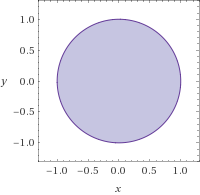
\includegraphics{image/3a}
			\label{fig:3a}
			
		\end{figure}
		
		\item $\{(x_1,x_2): 0 < x_1^2+x_2^2 \le 1 \} $ It is \textbf{not convex}. It excludes point [0, 0]
		\begin{figure}[h]
			\centering
			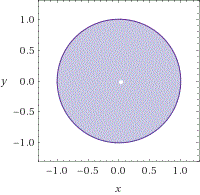
\includegraphics{image/3b}
			\label{fig:3b}
		\end{figure}
		
		\item $\{(x_1,x_2): |x_1|+|x_2| \le 1 \} $ It is \textbf{convex}.
		\begin{figure}[h]
			\centering
			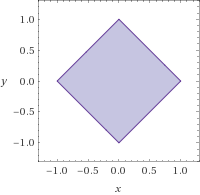
\includegraphics{image/3c}
			\label{fig:3b}
		\end{figure}
	\end{enumerate}

\end{homeworkProblem}

\begin{homeworkProblem}
	Let $C = \{x \in \R^n: Ax \le b\}$. Show that $C$ is a convex set.
	
	\textbf{Solution:}
	
	Let $x_1, x_2 \in C, \ 0\le \lambda \le 1$
	
	A convex combination is $ \lambda x_1 + (1-\lambda) x_2  $.
	\[ \begin{split}
	A(\lambda x_1 + (1-\lambda) x_2) 
	&= \lambda A x_1 + (1-\lambda) A x_2 \\
	&\le \lambda b + (1-\lambda) b \\
	&= b
	\end{split}	\]
	
\end{homeworkProblem}

\begin{homeworkProblem}[5]
	Show that the convex hull $H := conv S$ of a set $S \subseteq \R^n$ is the intersection of all convex sets $C$ that contain $S$, i.e., $H$ is equal to
	$\bigcap_{C\supseteq S,C convex} C =: M$.
	
	\textbf{Solution:}
	
	Take $x_1,x_2 \in S$, and $\lambda \in [0,1]$.
	
	Any convex combination 	$\lambda x_1 + (1-\lambda) x_2$ is in $H$, according to the definition of convex hull.  
	
	Let $C_i$ be a convex set containing all points in $S$.  Clearly $\lambda x_1 + (1-\lambda) x_2$ is in $C$, since $C$ is convex.  Therefore, all points in the convex hull, $H$, are in $C$.  Any such convex set $C_i \supseteq S$ will contain the convex hull $H$, so the intersection of all $C_i$ will also contain $H$. 
\end{homeworkProblem}



\begin{homeworkProblem}[6]
	What is the distance between two parallel hyperplanes $\{x \in \R^n: a^T x = b_1\}$ and $\{x \in \R^n: a^T x = b_2\}$
	
	\textbf{Solution:}
	
	Consider a point $x_1$ on the $b_1$ hyperplane.  A line normal to the $b_1$ hyperplane, passing through $x_1$, is defined by: $$x_1 + at; \ t \in \R$$
	
	The line intersects the $b_2$ hyperplane at a point $x_2$:
	
	$$a^T(x_1+at) = b_2$$
	$$a^T x_1 + a^T a t = b_2$$
	$$t = (b_2-b_1)/(a^T a) $$
	therefore
	$$ x_2 = x_1 + a\frac{b_2-b_1}{a^T a}$$
	and the distance between the hyperplanes is:
	\[ \begin{split} 
	\|x_1 - x_2\| &= \frac{|b_2-b_1|}{a^T a} \|a\| \\
				&= \frac{\abs{b_2-b_1}}{\|a\|^2} \|a\| \\
				&= \frac{\abs{b_2-b_1}}{\|a\|} 
	\end{split} \]
\end{homeworkProblem}


\begin{homeworkProblem}[7]
	
	
	\textbf{Solution:}
	
	
	
\end{homeworkProblem}


\begin{homeworkProblem}[8]
	Let $C \subseteq \R^n$ be the solution set of a quadratic inequality 
	$C = \{x \in \R^n: x^TAx + b^Tx+c \le 0 \}$	with $A\in S^n, S^n := \{M\in R^{n,n} : M=M^T \}$, $b\in \R^n$, $c\in \R$.  Show that $C$ is convex if $A$ is positive semi-definite.
	
	\textbf{Solution:}
	
	
	
	This set represents the sub-level set of a function.  Such a set is convex if the function is convex.   We know that a function is convex if $$f(\frac{x+y}{2}) \le \frac{1}{2}(f(x)+f(y)).$$  We need to prove that $f(x) = x^TAx + b^Tx+c$ is a convex function.
	
	Take $x,y \in \R^n$ ie: the domain of $f$. 
	
	\[\begin{split}
	\frac{1}{2}^2(x+y)^TA(x+y) + \frac{1}{2}b^T(x+y) + c &\stackrel{?}{\le} \frac{1}{2}(x^TAx+b^Ta+c+y^TAy+b^Ty+c)\\
	\frac{1}{2}^2(x+y)^TA(x+y) &\stackrel{?}{\le} \frac{1}{2}(x^TAx+y^TAy)\\
	x^TAx+y^TAy+x^TAy+y^TAx  &\stackrel{?}{\le} 2(x^TAx+y^TAy)\\
	0 &\stackrel{?}{\le} x^TAx+y^TAy-x^TAy-y^TAx\\
	0 &\stackrel{\checkmark}{\le} (x-y)^TA(x-y)\\
	\end{split} \]
	Because A is positive semi-definite.
	
	
\end{homeworkProblem}

\begin{homeworkProblem}[9]
	Determine which of the following sets are convex.
	\begin{enumerate}[a]
		\item The set $S = \{x \in \R^n: \alpha \le a^Tx \le \beta, \alpha,\beta \in \R, a\in \R^n      \}$
		\item The set of points closer to one set $S_1$ than another set $S_2$, i.e.,
		$$K = \{x \in \R^n : dist(x, S_1) \le dist(x, S_2)\} $$
		where $S_i \in \R^n$ and $dist(x, S) = \inf\{\|x-y\|_2 : y\in S\}$.
		\item The set of points whose distance to a point $x_0 \in \R^n$ does not exceed
		a fixed fraction $\alpha \in [0, 1]$ of the distance to $y \in \R^n, y \ne x_0$, i.e., the set $\{x \in \R^n : \|x - x_0\|_2 \le \alpha \|x - y\|_2\}$ .
	\end{enumerate}

	\textbf{Solution:}
	
	\begin{enumerate}[a]
		\item Yes, this is an intersection of two halfspaces, which we know to be convex from class.
		\item No, since the sets $S_1$ and $S_2$ are not specified to be convex, it is easy to construct a counter example.
		\begin{figure}[h]
			\centering
			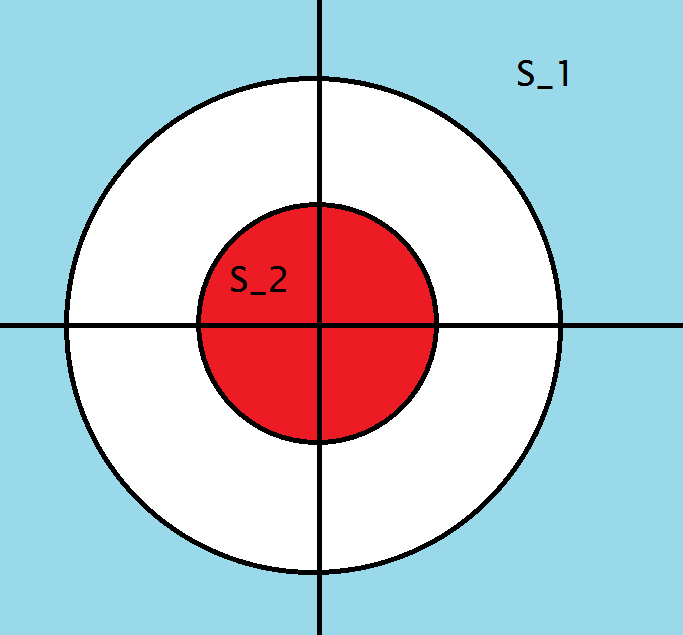
\includegraphics[width=0.3\linewidth]{image/9b}
			\caption{}
			\label{fig:9b}
		\end{figure}
		
		\item Yes, this defines a hypersphere (or n-ball), which is convex.  
	
	\end{enumerate}
	
\end{homeworkProblem}

\begin{homeworkProblem}[10]
	Let $S\subseteq \R^n$ and let $\|\cdot\|$ be some norm in $\R^n$.
	\begin{enumerate}[a]
		\item Let $S_\alpha := \{ x\in\R^n: dist(x,S)\le\alpha\}$, where $dist(x,S)=\inf_{y\in S}\|x-y\|$ with $\alpha \ge 0$. Show that if $S$ is convex, so is $S_\alpha$
		\item Let $S_{-\alpha} := \{ x\in\R^n:\B(x,\alpha) \subseteq S \}$, where $\B$ is the ball (in the norm  $\|\cdot\|$ ) centered around $x$ with radius $\alpha$. Show that if $S$ is convex, then $S_{-\alpha}$ is convex.
	\end{enumerate}
	
	\textbf{Solution:}
	
	\begin{enumerate}[a]
		\item 
		Let $x_1, x_2 \in S_\alpha\backslash S$, and $\lambda\in[0,1]$.
		
		Further, let $y_1, y_2$ be the closest points in $S$ to $x_1, x_2$, respectively. (ie: $y_1 = \arg\min_{y\in S}\|x_1-y\|$).
		
		Since $S$ is convex, we know that $y_c = \lambda y_1 + (1-\lambda)y_2$ is in $S$
		
		So let us consider the distance between $y_c$ and the convex combination in $S_\alpha$ defined by $x_c = \lambda x_1 + (1-\lambda)x_2$.
		\[ \begin{split}
		\|x_c - y_c\| &= \|(\lambda x_1 + (1-\lambda)x_2) - (\lambda y_1 + (1-\lambda)y_2) \| \\
		&=\|\lambda (x_1-y_1) + (1-\lambda)(x_2-y_2) \| 
		\shortintertext{by the triangle inequality, we have:}
		&\le  \|\lambda (x_1-y_1)\| + \|(1-\lambda)(x_2-y_2) \| \\
		&= \abs{\lambda}\|x_1-y_1\| +  \abs{1-\lambda}\|x_2-y_2\|\\
		&\le \lambda\alpha + (1-\lambda)\alpha\\
		&= \alpha
		\end{split} \]
		
		\item First, assume $S$ is convex.  Take $x_1 \ne x_2$ both $\in S$ such that 
		
		$ B_1 = \B(x_1,\alpha) \subseteq S $
		and $B_2 = \B(x_2, \alpha) \subseteq S$
		
		Consider two points $y_1 \in B_1$ and $y_2 \in B_2$.  Clearly, both $y_1, y_1 \in S$.  And since $S$ is convex, any point of the form $\lambda y_1 + (1-\lambda) y_2$ is in $S$ for $\lambda \in [0,1]$.  Therefore $S_{-\alpha}$ is convex.
	\end{enumerate}
\end{homeworkProblem}

\begin{homeworkProblem}[11]
	
	
	\textbf{Solution:}
	
	
	
\end{homeworkProblem}


\begin{homeworkProblem}[12]
	Let $C_i \subseteq \R^n$, $i = 1, 2$, be nonempty convex sets. Show that $S = \theta_1 C_1 + \theta_2 C_2$, where
	$$C_1 + C_2 := \{z \in\R^n : z = z_1 + z_2, z_1\in C_1, z_2 \in C_2\}$$
	is convex for any $\theta_i \in \R, i=1,2$.
	
	\textbf{Solution:}
	
	Let $u_1, u_2 \in S$.  \\
	That is: $u_1 = \theta_1 x_1 + \theta_2 y_1$ where $x_1\in C_1$ and $y_1 \in C_2$.  Similar definition for $u_2$.   \\
	Also let $\lambda \in [0,1]$.
	
	We show that a convex combination of $u_1$ and $u_2$ is in $S$.
	
	\[\begin{split}
	\lambda u_1 + (1-\lambda)u_2 &= \lambda(\theta_1 x_1 + \theta_2 y_1) + (1-\lambda)(\theta_1 x_2 + \theta_2 y_2)\\
	&= \lambda\theta_1x_1 + (1-\lambda)\theta_1x_2 + \lambda\theta_2y_1 + (1-\lambda)\theta_2y_2 \\
	&= \theta_1(\lambda x_1 + (1-\lambda)x_2) + \theta_2(\lambda y_1 + (1-\lambda)y_2)
	\end{split}\]
	And since $\lambda x_1 + (1-\lambda)x_2 \in C_1$ and $\lambda y_1 + (1-\lambda)y_2 \in C_2$, we have the desired result.
	
\end{homeworkProblem}

\begin{homeworkProblem}[13]
	
	
	\textbf{Solution:}
	
	
	
\end{homeworkProblem}

\end{document}
